\documentclass{article}
\usepackage{tikz}
\usetikzlibrary{shapes,arrows}

\begin{document}

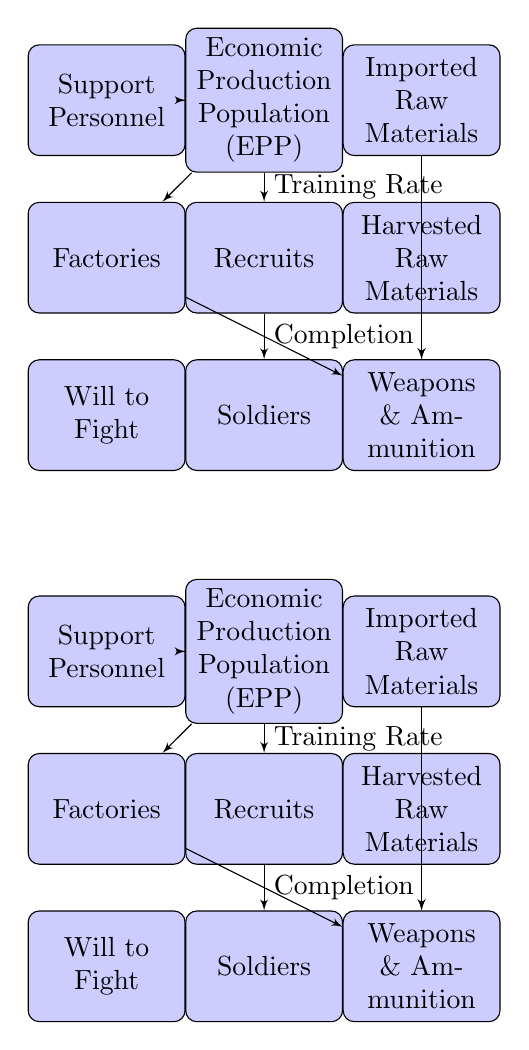
\begin{tikzpicture}[node distance = 2cm, auto]
    % Define block styles
    \tikzstyle{block} = [rectangle, draw, fill=blue!20,
        text width=5em, text centered, rounded corners, minimum height=4em]
    \tikzstyle{line} = [draw, -latex']

    % State A
    \node [block] (eppA) {Economic Production Population (EPP)};
    \node [block, below of=eppA] (recruitsA) {Recruits};
    \node [block, below of=recruitsA] (soldiersA) {Soldiers};
    \node [block, right of=eppA] (importA) {Imported Raw Materials};
    \node [block, right of=recruitsA] (harvestA) {Harvested Raw Materials};
    \node [block, right of=soldiersA] (weaponsA) {Weapons \& Ammunition};
    \node [block, left of=eppA] (supportA) {Support Personnel};
    \node [block, left of=recruitsA] (factoriesA) {Factories};
    \node [block, left of=soldiersA] (willA) {Will to Fight};

    % State A paths
    \path [line] (eppA) -- node {Training Rate} (recruitsA);
    \path [line] (recruitsA) -- node {Completion} (soldiersA);
    \path [line] (importA) -- (weaponsA);
    \path [line] (harvestA) -- (weaponsA);
    \path [line] (eppA) -- (supportA);
    \path [line] (eppA) -- (factoriesA);
    \path [line] (factoriesA) -- (weaponsA);

    % State B (positioned relative to State A for clarity)
    \node [block, below of=soldiersA, node distance=3cm] (eppB) {Economic Production Population (EPP)};
    \node [block, below of=eppB] (recruitsB) {Recruits};
    \node [block, below of=recruitsB] (soldiersB) {Soldiers};
    \node [block, right of=eppB] (importB) {Imported Raw Materials};
    \node [block, right of=recruitsB] (harvestB) {Harvested Raw Materials};
    \node [block, right of=soldiersB] (weaponsB) {Weapons \& Ammunition};
    \node [block, left of=eppB] (supportB) {Support Personnel};
    \node [block, left of=recruitsB] (factoriesB) {Factories};
    \node [block, left of=soldiersB] (willB) {Will to Fight};

    % State B paths
    \path [line] (eppB) -- node {Training Rate} (recruitsB);
    \path [line] (recruitsB) -- node {Completion} (soldiersB);
    \path [line] (importB) -- (weaponsB);
    \path [line] (harvestB) -- (weaponsB);
    \path [line] (eppB) -- (supportB);
    \path [line] (eppB) -- (factoriesB);
    \path [line] (factoriesB) -- (weaponsB);

\end{tikzpicture}

\end{document}
